\documentclass[twoside]{book}

% Packages required by doxygen
\usepackage{fixltx2e}
\usepackage{calc}
\usepackage{doxygen}
\usepackage[export]{adjustbox} % also loads graphicx
\usepackage{graphicx}
\usepackage[utf8]{inputenc}
\usepackage{makeidx}
\usepackage{multicol}
\usepackage{multirow}
\PassOptionsToPackage{warn}{textcomp}
\usepackage{textcomp}
\usepackage[nointegrals]{wasysym}
\usepackage[table]{xcolor}

% Font selection
\usepackage[T1]{fontenc}
\usepackage[scaled=.90]{helvet}
\usepackage{courier}
\usepackage{amssymb}
\usepackage{sectsty}
\renewcommand{\familydefault}{\sfdefault}
\allsectionsfont{%
  \fontseries{bc}\selectfont%
  \color{darkgray}%
}
\renewcommand{\DoxyLabelFont}{%
  \fontseries{bc}\selectfont%
  \color{darkgray}%
}
\newcommand{\+}{\discretionary{\mbox{\scriptsize$\hookleftarrow$}}{}{}}

% Page & text layout
\usepackage{geometry}
\geometry{%
  a4paper,%
  top=2.5cm,%
  bottom=2.5cm,%
  left=2.5cm,%
  right=2.5cm%
}
\tolerance=750
\hfuzz=15pt
\hbadness=750
\setlength{\emergencystretch}{15pt}
\setlength{\parindent}{0cm}
\setlength{\parskip}{3ex plus 2ex minus 2ex}
\makeatletter
\renewcommand{\paragraph}{%
  \@startsection{paragraph}{4}{0ex}{-1.0ex}{1.0ex}{%
    \normalfont\normalsize\bfseries\SS@parafont%
  }%
}
\renewcommand{\subparagraph}{%
  \@startsection{subparagraph}{5}{0ex}{-1.0ex}{1.0ex}{%
    \normalfont\normalsize\bfseries\SS@subparafont%
  }%
}
\makeatother

% Headers & footers
\usepackage{fancyhdr}
\pagestyle{fancyplain}
\fancyhead[LE]{\fancyplain{}{\bfseries\thepage}}
\fancyhead[CE]{\fancyplain{}{}}
\fancyhead[RE]{\fancyplain{}{\bfseries\leftmark}}
\fancyhead[LO]{\fancyplain{}{\bfseries\rightmark}}
\fancyhead[CO]{\fancyplain{}{}}
\fancyhead[RO]{\fancyplain{}{\bfseries\thepage}}
\fancyfoot[LE]{\fancyplain{}{}}
\fancyfoot[CE]{\fancyplain{}{}}
\fancyfoot[RE]{\fancyplain{}{\bfseries\scriptsize Generated by Doxygen }}
\fancyfoot[LO]{\fancyplain{}{\bfseries\scriptsize Generated by Doxygen }}
\fancyfoot[CO]{\fancyplain{}{}}
\fancyfoot[RO]{\fancyplain{}{}}
\renewcommand{\footrulewidth}{0.4pt}
\renewcommand{\chaptermark}[1]{%
  \markboth{#1}{}%
}
\renewcommand{\sectionmark}[1]{%
  \markright{\thesection\ #1}%
}

% Indices & bibliography
\usepackage{natbib}
\usepackage[titles]{tocloft}
\setcounter{tocdepth}{3}
\setcounter{secnumdepth}{5}
\makeindex

% Hyperlinks (required, but should be loaded last)
\usepackage{ifpdf}
\ifpdf
  \usepackage[pdftex,pagebackref=true]{hyperref}
\else
  \usepackage[ps2pdf,pagebackref=true]{hyperref}
\fi
\hypersetup{%
  colorlinks=true,%
  linkcolor=blue,%
  citecolor=blue,%
  unicode%
}

% Custom commands
\newcommand{\clearemptydoublepage}{%
  \newpage{\pagestyle{empty}\cleardoublepage}%
}

\usepackage{caption}
\captionsetup{labelsep=space,justification=centering,font={bf},singlelinecheck=off,skip=4pt,position=top}

%===== C O N T E N T S =====

\begin{document}

% Titlepage & ToC
\hypersetup{pageanchor=false,
             bookmarksnumbered=true,
             pdfencoding=unicode
            }
\pagenumbering{roman}
\begin{titlepage}
\vspace*{7cm}
\begin{center}%
{\Large Android\+Mouse \\[1ex]\large 1.\+0 }\\
\vspace*{1cm}
{\large Generated by Doxygen 1.8.11}\\
\end{center}
\end{titlepage}
\clearemptydoublepage
\tableofcontents
\clearemptydoublepage
\pagenumbering{arabic}
\hypersetup{pageanchor=true}

%--- Begin generated contents ---
\chapter{R\+E\+A\+D\+ME}
\label{md_README}
\hypertarget{md_README}{}
\#\+Project 3

For project 3, I am creating an Android app that will allow a user to control a computer mouse cursor by tilting the android device. To do this, the Android device will collect orientation readings from its I\+MU sensor. The device’s y-\/axis rotation will be used to move the cursor left and right, while its x-\/axis rotation will be used to move the cursor up and down. If this is accomplished successfully, I will attempt to implement additional features, such as left and right click using touch buttons. The app will perform a simple filter on this data and send values over a network socket to a server hosted on the target computer. On the server side, a java program will receive messages from the Android device and store them in a buffer. The program will then parse the message and determine what mouse action is to be performed. The actions will be performed using Java’s Abstract Window Toolkit. The mouse cursor speed will be determined by the rotation data sent by the phone, and the cursor acceleration will be limited by the data filtering.

\subsubsection*{4/8 P\+R\+O\+G\+R\+E\+SS R\+E\+P\+O\+RT}

As of today I have set up the basic architecture of the app. It can collect rotation data, although this was kind of trivial. I have been trying to get the app to connect to a server on my computer. However, I have not been able to attempt the connection without the app crashing. 
\chapter{Namespace Index}
\section{Packages}
Here are the packages with brief descriptions (if available)\+:\begin{DoxyCompactList}
\item\contentsline{section}{\hyperlink{namespaceio_1_1github_1_1samshore_1_1clientapp}{io.\+github.\+samshore.\+clientapp} \\*Automatically generated file }{\pageref{namespaceio_1_1github_1_1samshore_1_1clientapp}}{}
\item\contentsline{section}{\hyperlink{namespaceio_1_1github_1_1samshore_1_1clientapp_1_1test}{io.\+github.\+samshore.\+clientapp.\+test} \\*Automatically generated file }{\pageref{namespaceio_1_1github_1_1samshore_1_1clientapp_1_1test}}{}
\end{DoxyCompactList}

\chapter{Hierarchical Index}
\section{Class Hierarchy}
This inheritance list is sorted roughly, but not completely, alphabetically\+:\begin{DoxyCompactList}
\item \contentsline{section}{edu.\+tamu.\+rfsignalmap.\+Lat\+Long}{\pageref{classedu_1_1tamu_1_1rfsignalmap_1_1_lat_long}}{}
\item On\+Click\+Listener\begin{DoxyCompactList}
\item \contentsline{section}{edu.\+tamu.\+rfsignalmap.\+Main\+Activity\+Fragment}{\pageref{classedu_1_1tamu_1_1rfsignalmap_1_1_main_activity_fragment}}{}
\end{DoxyCompactList}
\item On\+Preference\+Change\+Listener\begin{DoxyCompactList}
\item \contentsline{section}{edu.\+tamu.\+rfsignalmap.\+Settings\+Fragment}{\pageref{classedu_1_1tamu_1_1rfsignalmap_1_1_settings_fragment}}{}
\end{DoxyCompactList}
\item \contentsline{section}{edu.\+tamu.\+rfsignalmap.\+R\+F\+Data}{\pageref{classedu_1_1tamu_1_1rfsignalmap_1_1_r_f_data}}{}
\item \contentsline{section}{edu.\+tamu.\+rfsignalmap.\+R\+F\+Field\+S\+Q\+L\+Database}{\pageref{classedu_1_1tamu_1_1rfsignalmap_1_1_r_f_field_s_q_l_database}}{}
\item App\+Compat\+Activity\begin{DoxyCompactList}
\item \contentsline{section}{edu.\+tamu.\+rfsignalmap.\+Main\+Activity}{\pageref{classedu_1_1tamu_1_1rfsignalmap_1_1_main_activity}}{}
\end{DoxyCompactList}
\item Fragment\begin{DoxyCompactList}
\item \contentsline{section}{edu.\+tamu.\+rfsignalmap.\+About\+Fragment}{\pageref{classedu_1_1tamu_1_1rfsignalmap_1_1_about_fragment}}{}
\item \contentsline{section}{edu.\+tamu.\+rfsignalmap.\+Main\+Activity\+Fragment}{\pageref{classedu_1_1tamu_1_1rfsignalmap_1_1_main_activity_fragment}}{}
\item \contentsline{section}{edu.\+tamu.\+rfsignalmap.\+Maps\+View\+Fragment}{\pageref{classedu_1_1tamu_1_1rfsignalmap_1_1_maps_view_fragment}}{}
\end{DoxyCompactList}
\item Location\+Listener\begin{DoxyCompactList}
\item \contentsline{section}{edu.\+tamu.\+rfsignalmap.\+Main\+Activity\+Fragment}{\pageref{classedu_1_1tamu_1_1rfsignalmap_1_1_main_activity_fragment}}{}
\end{DoxyCompactList}
\item On\+Map\+Click\+Listener\begin{DoxyCompactList}
\item \contentsline{section}{edu.\+tamu.\+rfsignalmap.\+Maps\+View\+Fragment}{\pageref{classedu_1_1tamu_1_1rfsignalmap_1_1_maps_view_fragment}}{}
\end{DoxyCompactList}
\item On\+Map\+Ready\+Callback\begin{DoxyCompactList}
\item \contentsline{section}{edu.\+tamu.\+rfsignalmap.\+Maps\+View\+Fragment}{\pageref{classedu_1_1tamu_1_1rfsignalmap_1_1_maps_view_fragment}}{}
\end{DoxyCompactList}
\item Preference\+Fragment\begin{DoxyCompactList}
\item \contentsline{section}{edu.\+tamu.\+rfsignalmap.\+Settings\+Fragment}{\pageref{classedu_1_1tamu_1_1rfsignalmap_1_1_settings_fragment}}{}
\end{DoxyCompactList}
\item Sensor\+Event\+Listener\begin{DoxyCompactList}
\item \contentsline{section}{edu.\+tamu.\+rfsignalmap.\+Main\+Activity\+Fragment}{\pageref{classedu_1_1tamu_1_1rfsignalmap_1_1_main_activity_fragment}}{}
\end{DoxyCompactList}
\end{DoxyCompactList}

\chapter{Class Index}
\section{Class List}
Here are the classes, structs, unions and interfaces with brief descriptions\+:\begin{DoxyCompactList}
\item\contentsline{section}{\hyperlink{classedu_1_1tamu_1_1rfsignalmap_1_1_about_fragment}{edu.\+tamu.\+rfsignalmap.\+About\+Fragment} \\*About Fragment -\/ Application Information }{\pageref{classedu_1_1tamu_1_1rfsignalmap_1_1_about_fragment}}{}
\item\contentsline{section}{\hyperlink{classedu_1_1tamu_1_1rfsignalmap_1_1_lat_long}{edu.\+tamu.\+rfsignalmap.\+Lat\+Long} \\*\hyperlink{classedu_1_1tamu_1_1rfsignalmap_1_1_lat_long}{Lat\+Long} class -\/ \hyperlink{classedu_1_1tamu_1_1rfsignalmap_1_1_lat_long}{Lat\+Long} Field Data }{\pageref{classedu_1_1tamu_1_1rfsignalmap_1_1_lat_long}}{}
\item\contentsline{section}{\hyperlink{classedu_1_1tamu_1_1rfsignalmap_1_1_main_activity}{edu.\+tamu.\+rfsignalmap.\+Main\+Activity} \\*Main Activity Application Project }{\pageref{classedu_1_1tamu_1_1rfsignalmap_1_1_main_activity}}{}
\item\contentsline{section}{\hyperlink{classedu_1_1tamu_1_1rfsignalmap_1_1_main_activity_fragment}{edu.\+tamu.\+rfsignalmap.\+Main\+Activity\+Fragment} \\*Main Activity Fragment -\/ Display Captured Data }{\pageref{classedu_1_1tamu_1_1rfsignalmap_1_1_main_activity_fragment}}{}
\item\contentsline{section}{\hyperlink{classedu_1_1tamu_1_1rfsignalmap_1_1_maps_view_fragment}{edu.\+tamu.\+rfsignalmap.\+Maps\+View\+Fragment} \\*Maps View Fragment for Application Project }{\pageref{classedu_1_1tamu_1_1rfsignalmap_1_1_maps_view_fragment}}{}
\item\contentsline{section}{\hyperlink{classedu_1_1tamu_1_1rfsignalmap_1_1_r_f_data}{edu.\+tamu.\+rfsignalmap.\+R\+F\+Data} \\*\hyperlink{classedu_1_1tamu_1_1rfsignalmap_1_1_r_f_data}{R\+F\+Data} class -\/ RF Field Data w/ J\+S\+ON support }{\pageref{classedu_1_1tamu_1_1rfsignalmap_1_1_r_f_data}}{}
\item\contentsline{section}{\hyperlink{classedu_1_1tamu_1_1rfsignalmap_1_1_r_f_field_s_q_l_database}{edu.\+tamu.\+rfsignalmap.\+R\+F\+Field\+S\+Q\+L\+Database} \\*\hyperlink{classedu_1_1tamu_1_1rfsignalmap_1_1_r_f_field_s_q_l_database}{R\+F\+Field\+S\+Q\+L\+Database} interfaces S\+QL Database, supplies methods to access data and passes }{\pageref{classedu_1_1tamu_1_1rfsignalmap_1_1_r_f_field_s_q_l_database}}{}
\item\contentsline{section}{\hyperlink{classedu_1_1tamu_1_1rfsignalmap_1_1_settings_fragment}{edu.\+tamu.\+rfsignalmap.\+Settings\+Fragment} \\*Settings Fragment -\/ Application Information }{\pageref{classedu_1_1tamu_1_1rfsignalmap_1_1_settings_fragment}}{}
\end{DoxyCompactList}

\chapter{Namespace Documentation}
\hypertarget{namespaceio_1_1github_1_1samshore_1_1clientapp}{}\section{Package io.\+github.\+samshore.\+clientapp}
\label{namespaceio_1_1github_1_1samshore_1_1clientapp}\index{io.\+github.\+samshore.\+clientapp@{io.\+github.\+samshore.\+clientapp}}


Automatically generated file.  


\subsection*{Packages}
\begin{DoxyCompactItemize}
\item 
package \hyperlink{namespaceio_1_1github_1_1samshore_1_1clientapp_1_1test}{test}
\begin{DoxyCompactList}\small\item\em Automatically generated file. \end{DoxyCompactList}\end{DoxyCompactItemize}
\subsection*{Classes}
\begin{DoxyCompactItemize}
\item 
class \hyperlink{classio_1_1github_1_1samshore_1_1clientapp_1_1_application_test}{Application\+Test}
\begin{DoxyCompactList}\small\item\em \href{http://d.android.com/tools/testing/testing_android.html}{\tt Testing Fundamentals} \end{DoxyCompactList}\item 
class \hyperlink{classio_1_1github_1_1samshore_1_1clientapp_1_1_build_config}{Build\+Config}
\item 
class \hyperlink{classio_1_1github_1_1samshore_1_1clientapp_1_1_example_unit_test}{Example\+Unit\+Test}
\begin{DoxyCompactList}\small\item\em To work on unit tests, switch the Test Artifact in the Build Variants view. \end{DoxyCompactList}\item 
class \hyperlink{classio_1_1github_1_1samshore_1_1clientapp_1_1_main_activity}{Main\+Activity}
\begin{DoxyCompactList}\small\item\em \hyperlink{classio_1_1github_1_1samshore_1_1clientapp_1_1_main_activity}{Main\+Activity}. \end{DoxyCompactList}\item 
class \hyperlink{classio_1_1github_1_1samshore_1_1clientapp_1_1_r}{R}
\end{DoxyCompactItemize}


\subsection{Detailed Description}
Automatically generated file. 

DO N\+OT M\+O\+D\+I\+FY 
\hypertarget{namespaceio_1_1github_1_1samshore_1_1clientapp_1_1test}{}\section{Package io.\+github.\+samshore.\+clientapp.\+test}
\label{namespaceio_1_1github_1_1samshore_1_1clientapp_1_1test}\index{io.\+github.\+samshore.\+clientapp.\+test@{io.\+github.\+samshore.\+clientapp.\+test}}


Automatically generated file.  


\subsection*{Classes}
\begin{DoxyCompactItemize}
\item 
class \hyperlink{classio_1_1github_1_1samshore_1_1clientapp_1_1test_1_1_build_config}{Build\+Config}
\end{DoxyCompactItemize}


\subsection{Detailed Description}
Automatically generated file. 

DO N\+OT M\+O\+D\+I\+FY 
\chapter{Class Documentation}
\hypertarget{classio_1_1github_1_1samshore_1_1clientapp_1_1_application_test}{}\section{io.\+github.\+samshore.\+clientapp.\+Application\+Test Class Reference}
\label{classio_1_1github_1_1samshore_1_1clientapp_1_1_application_test}\index{io.\+github.\+samshore.\+clientapp.\+Application\+Test@{io.\+github.\+samshore.\+clientapp.\+Application\+Test}}


\href{http://d.android.com/tools/testing/testing_android.html}{\tt Testing Fundamentals}  


Inheritance diagram for io.\+github.\+samshore.\+clientapp.\+Application\+Test\+:\begin{figure}[H]
\begin{center}
\leavevmode
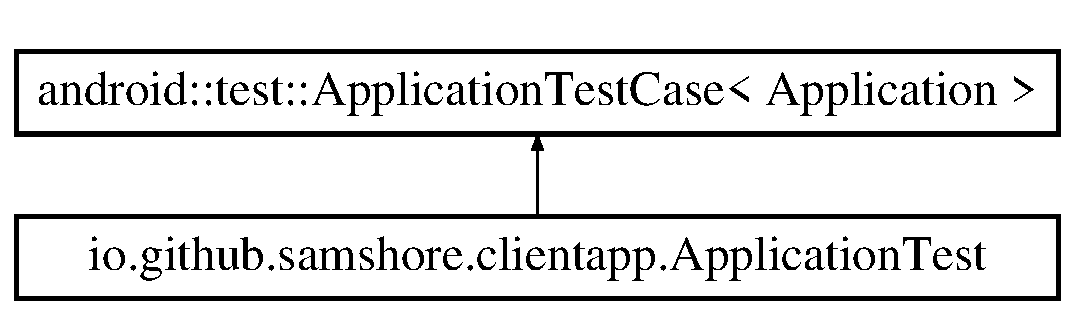
\includegraphics[height=2.000000cm]{classio_1_1github_1_1samshore_1_1clientapp_1_1_application_test}
\end{center}
\end{figure}


\subsection{Detailed Description}
\href{http://d.android.com/tools/testing/testing_android.html}{\tt Testing Fundamentals} 

The documentation for this class was generated from the following file\+:\begin{DoxyCompactItemize}
\item 
Client\+App/app/src/android\+Test/java/io/github/samshore/clientapp/Application\+Test.\+java\end{DoxyCompactItemize}

\hypertarget{classio_1_1github_1_1samshore_1_1clientapp_1_1test_1_1_build_config}{}\section{io.\+github.\+samshore.\+clientapp.\+test.\+Build\+Config Class Reference}
\label{classio_1_1github_1_1samshore_1_1clientapp_1_1test_1_1_build_config}\index{io.\+github.\+samshore.\+clientapp.\+test.\+Build\+Config@{io.\+github.\+samshore.\+clientapp.\+test.\+Build\+Config}}
\subsection*{Static Public Attributes}
\begin{DoxyCompactItemize}
\item 
static final boolean {\bfseries D\+E\+B\+UG} = Boolean.\+parse\+Boolean(\char`\"{}true\char`\"{})\hypertarget{classio_1_1github_1_1samshore_1_1clientapp_1_1test_1_1_build_config_a5eb8217951dc63eeb07b39a3cccb56eb}{}\label{classio_1_1github_1_1samshore_1_1clientapp_1_1test_1_1_build_config_a5eb8217951dc63eeb07b39a3cccb56eb}

\item 
static final String {\bfseries A\+P\+P\+L\+I\+C\+A\+T\+I\+O\+N\+\_\+\+ID} = \char`\"{}io.\+github.\+samshore.\+clientapp.\+test\char`\"{}\hypertarget{classio_1_1github_1_1samshore_1_1clientapp_1_1test_1_1_build_config_ae798e12ed2e750037f4030f74a3abce2}{}\label{classio_1_1github_1_1samshore_1_1clientapp_1_1test_1_1_build_config_ae798e12ed2e750037f4030f74a3abce2}

\item 
static final String {\bfseries B\+U\+I\+L\+D\+\_\+\+T\+Y\+PE} = \char`\"{}debug\char`\"{}\hypertarget{classio_1_1github_1_1samshore_1_1clientapp_1_1test_1_1_build_config_a2d9c2243494dca9eb531b28ab2913564}{}\label{classio_1_1github_1_1samshore_1_1clientapp_1_1test_1_1_build_config_a2d9c2243494dca9eb531b28ab2913564}

\item 
static final String {\bfseries F\+L\+A\+V\+OR} = \char`\"{}\char`\"{}\hypertarget{classio_1_1github_1_1samshore_1_1clientapp_1_1test_1_1_build_config_af5e46e2dd446ca0f4ce0f7c4fedf71c0}{}\label{classio_1_1github_1_1samshore_1_1clientapp_1_1test_1_1_build_config_af5e46e2dd446ca0f4ce0f7c4fedf71c0}

\item 
static final int {\bfseries V\+E\+R\+S\+I\+O\+N\+\_\+\+C\+O\+DE} = 1\hypertarget{classio_1_1github_1_1samshore_1_1clientapp_1_1test_1_1_build_config_aeef1852bd07ffba1f50a17437119ea8d}{}\label{classio_1_1github_1_1samshore_1_1clientapp_1_1test_1_1_build_config_aeef1852bd07ffba1f50a17437119ea8d}

\item 
static final String {\bfseries V\+E\+R\+S\+I\+O\+N\+\_\+\+N\+A\+ME} = \char`\"{}1.\+0\char`\"{}\hypertarget{classio_1_1github_1_1samshore_1_1clientapp_1_1test_1_1_build_config_a994e4734b6d3c46645616cb18d1b9e95}{}\label{classio_1_1github_1_1samshore_1_1clientapp_1_1test_1_1_build_config_a994e4734b6d3c46645616cb18d1b9e95}

\end{DoxyCompactItemize}


The documentation for this class was generated from the following file\+:\begin{DoxyCompactItemize}
\item 
Client\+App/app/build/generated/source/build\+Config/android\+Test/debug/io/github/samshore/clientapp/test/Build\+Config.\+java\end{DoxyCompactItemize}

\hypertarget{classio_1_1github_1_1samshore_1_1clientapp_1_1_build_config}{}\section{io.\+github.\+samshore.\+clientapp.\+Build\+Config Class Reference}
\label{classio_1_1github_1_1samshore_1_1clientapp_1_1_build_config}\index{io.\+github.\+samshore.\+clientapp.\+Build\+Config@{io.\+github.\+samshore.\+clientapp.\+Build\+Config}}
\subsection*{Static Public Attributes}
\begin{DoxyCompactItemize}
\item 
static final boolean {\bfseries D\+E\+B\+UG} = Boolean.\+parse\+Boolean(\char`\"{}true\char`\"{})\hypertarget{classio_1_1github_1_1samshore_1_1clientapp_1_1_build_config_a6723df3a1d3832e6db22ef99269c3576}{}\label{classio_1_1github_1_1samshore_1_1clientapp_1_1_build_config_a6723df3a1d3832e6db22ef99269c3576}

\item 
static final String {\bfseries A\+P\+P\+L\+I\+C\+A\+T\+I\+O\+N\+\_\+\+ID} = \char`\"{}io.\+github.\+samshore.\+clientapp\char`\"{}\hypertarget{classio_1_1github_1_1samshore_1_1clientapp_1_1_build_config_a25af248e8420161c04e6e9c70df93e32}{}\label{classio_1_1github_1_1samshore_1_1clientapp_1_1_build_config_a25af248e8420161c04e6e9c70df93e32}

\item 
static final String {\bfseries B\+U\+I\+L\+D\+\_\+\+T\+Y\+PE} = \char`\"{}debug\char`\"{}\hypertarget{classio_1_1github_1_1samshore_1_1clientapp_1_1_build_config_a5b0d3d986a05b1abbe079182900650f8}{}\label{classio_1_1github_1_1samshore_1_1clientapp_1_1_build_config_a5b0d3d986a05b1abbe079182900650f8}

\item 
static final String {\bfseries F\+L\+A\+V\+OR} = \char`\"{}\char`\"{}\hypertarget{classio_1_1github_1_1samshore_1_1clientapp_1_1_build_config_a6512f075334cee2d1d0d868cff6843e4}{}\label{classio_1_1github_1_1samshore_1_1clientapp_1_1_build_config_a6512f075334cee2d1d0d868cff6843e4}

\item 
static final int {\bfseries V\+E\+R\+S\+I\+O\+N\+\_\+\+C\+O\+DE} = 1\hypertarget{classio_1_1github_1_1samshore_1_1clientapp_1_1_build_config_ae128ad13fbd0ef6a97068aba166f5dad}{}\label{classio_1_1github_1_1samshore_1_1clientapp_1_1_build_config_ae128ad13fbd0ef6a97068aba166f5dad}

\item 
static final String {\bfseries V\+E\+R\+S\+I\+O\+N\+\_\+\+N\+A\+ME} = \char`\"{}1.\+0\char`\"{}\hypertarget{classio_1_1github_1_1samshore_1_1clientapp_1_1_build_config_a6d624de812b2bcebfd84791d1c7c3b78}{}\label{classio_1_1github_1_1samshore_1_1clientapp_1_1_build_config_a6d624de812b2bcebfd84791d1c7c3b78}

\end{DoxyCompactItemize}


The documentation for this class was generated from the following file\+:\begin{DoxyCompactItemize}
\item 
Client\+App/app/build/generated/source/build\+Config/debug/io/github/samshore/clientapp/Build\+Config.\+java\end{DoxyCompactItemize}

\hypertarget{class_cursor_thread}{}\section{Cursor\+Thread Class Reference}
\label{class_cursor_thread}\index{Cursor\+Thread@{Cursor\+Thread}}


\hyperlink{class_cursor_thread}{Cursor\+Thread} class.  


Inheritance diagram for Cursor\+Thread\+:\begin{figure}[H]
\begin{center}
\leavevmode
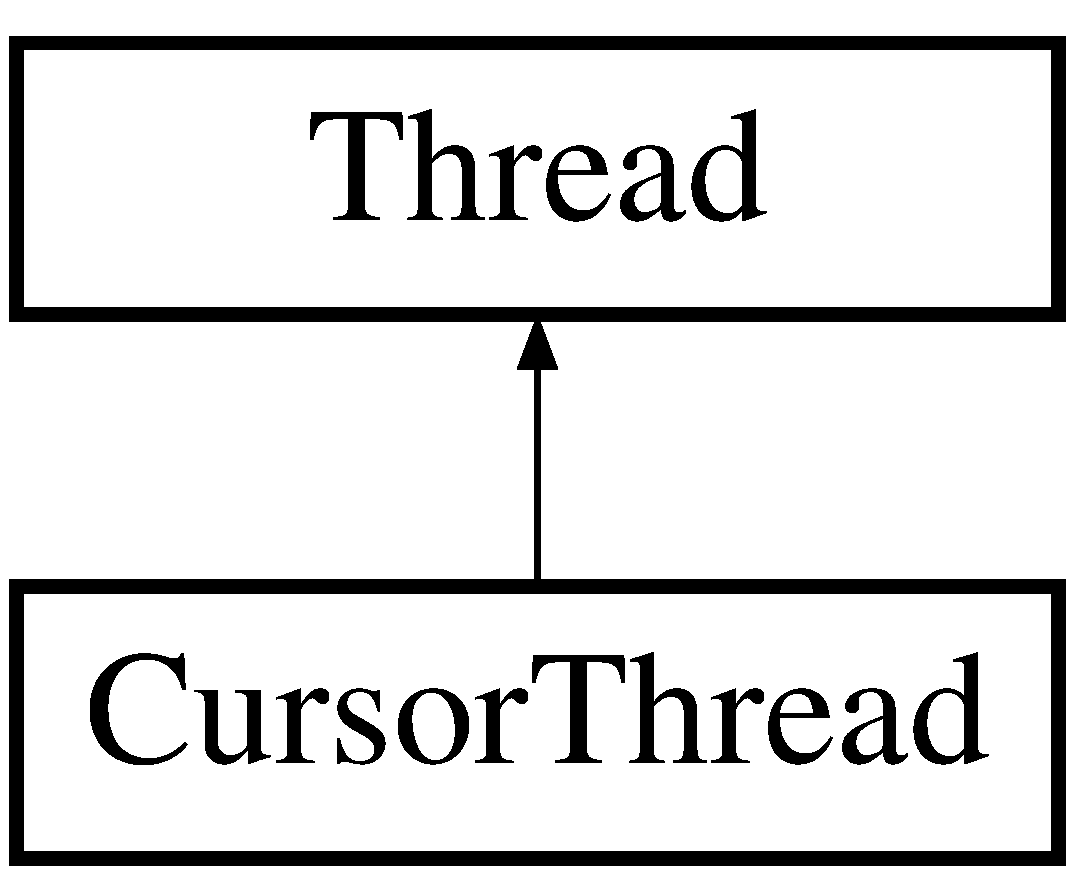
\includegraphics[height=2.000000cm]{class_cursor_thread}
\end{center}
\end{figure}
\subsection*{Public Member Functions}
\begin{DoxyCompactItemize}
\item 
void {\bfseries run} ()\hypertarget{class_cursor_thread_a9301a34692a1b3c3387e82f4c463fcb2}{}\label{class_cursor_thread_a9301a34692a1b3c3387e82f4c463fcb2}

\item 
void {\bfseries start} ()\hypertarget{class_cursor_thread_a4c40d058f6b9b5f95c6c68db44fb5a26}{}\label{class_cursor_thread_a4c40d058f6b9b5f95c6c68db44fb5a26}

\end{DoxyCompactItemize}
\subsection*{Public Attributes}
\begin{DoxyCompactItemize}
\item 
Dimension {\bfseries screen\+Size} = Toolkit.\+get\+Default\+Toolkit().get\+Screen\+Size()\hypertarget{class_cursor_thread_aa502eaff9091012ae0e8eb5ec85fa551}{}\label{class_cursor_thread_aa502eaff9091012ae0e8eb5ec85fa551}

\item 
double {\bfseries width} = screen\+Size.\+get\+Width()\hypertarget{class_cursor_thread_a44f7c6590e5893a54824cf3d3a4e2bcb}{}\label{class_cursor_thread_a44f7c6590e5893a54824cf3d3a4e2bcb}

\item 
double {\bfseries height} = screen\+Size.\+get\+Height()\hypertarget{class_cursor_thread_af3bfed280e640ba1a55b49a0d3f48755}{}\label{class_cursor_thread_af3bfed280e640ba1a55b49a0d3f48755}

\item 
int {\bfseries current\+PosX} = (int)Math.\+round(width/2)\hypertarget{class_cursor_thread_a4f68655ab65b581c5194f75f2510c866}{}\label{class_cursor_thread_a4f68655ab65b581c5194f75f2510c866}

\item 
int {\bfseries current\+PosY} = (int)Math.\+round(height/2)\hypertarget{class_cursor_thread_a3e1987c0d9d200e1022e1ca4885e3cfb}{}\label{class_cursor_thread_a3e1987c0d9d200e1022e1ca4885e3cfb}

\end{DoxyCompactItemize}


\subsection{Detailed Description}
\hyperlink{class_cursor_thread}{Cursor\+Thread} class. 

Takes the rotation information and performs simple calculations to create a cursor offset. This offset is added to the cursor\textquotesingle{}s current postion. The cursor is moved to this new coordinate using Java\textquotesingle{}s abstract window toolkit. 

The documentation for this class was generated from the following file\+:\begin{DoxyCompactItemize}
\item 
Android\+Mouse/src/Cursor\+Thread.\+java\end{DoxyCompactItemize}

\hypertarget{classio_1_1github_1_1samshore_1_1clientapp_1_1_example_unit_test}{}\section{io.\+github.\+samshore.\+clientapp.\+Example\+Unit\+Test Class Reference}
\label{classio_1_1github_1_1samshore_1_1clientapp_1_1_example_unit_test}\index{io.\+github.\+samshore.\+clientapp.\+Example\+Unit\+Test@{io.\+github.\+samshore.\+clientapp.\+Example\+Unit\+Test}}


To work on unit tests, switch the Test Artifact in the Build Variants view.  


\subsection*{Public Member Functions}
\begin{DoxyCompactItemize}
\item 
void {\bfseries addition\+\_\+is\+Correct} ()  throws Exception \hypertarget{classio_1_1github_1_1samshore_1_1clientapp_1_1_example_unit_test_a7dda2578c57f518bdec36eaa97ea917b}{}\label{classio_1_1github_1_1samshore_1_1clientapp_1_1_example_unit_test_a7dda2578c57f518bdec36eaa97ea917b}

\end{DoxyCompactItemize}


\subsection{Detailed Description}
To work on unit tests, switch the Test Artifact in the Build Variants view. 

The documentation for this class was generated from the following file\+:\begin{DoxyCompactItemize}
\item 
Client\+App/app/src/test/java/io/github/samshore/clientapp/Example\+Unit\+Test.\+java\end{DoxyCompactItemize}

\hypertarget{classio_1_1github_1_1samshore_1_1clientapp_1_1_main_activity}{}\section{io.\+github.\+samshore.\+clientapp.\+Main\+Activity Class Reference}
\label{classio_1_1github_1_1samshore_1_1clientapp_1_1_main_activity}\index{io.\+github.\+samshore.\+clientapp.\+Main\+Activity@{io.\+github.\+samshore.\+clientapp.\+Main\+Activity}}


\hyperlink{classio_1_1github_1_1samshore_1_1clientapp_1_1_main_activity}{Main\+Activity}.  


Inheritance diagram for io.\+github.\+samshore.\+clientapp.\+Main\+Activity\+:\begin{figure}[H]
\begin{center}
\leavevmode
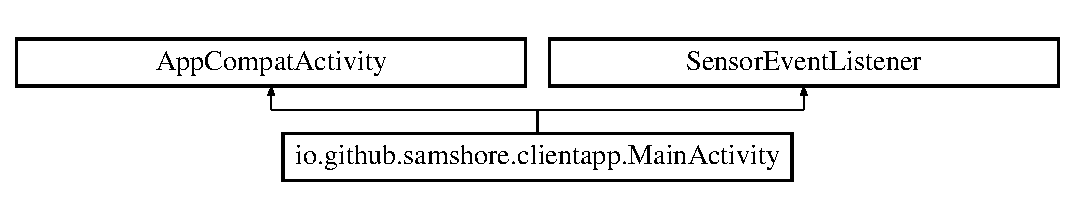
\includegraphics[height=2.000000cm]{classio_1_1github_1_1samshore_1_1clientapp_1_1_main_activity}
\end{center}
\end{figure}
\subsection*{Public Member Functions}
\begin{DoxyCompactItemize}
\item 
boolean {\bfseries on\+Create\+Options\+Menu} (Menu menu)\hypertarget{classio_1_1github_1_1samshore_1_1clientapp_1_1_main_activity_a4b07c90c6171135421905a0d56326c77}{}\label{classio_1_1github_1_1samshore_1_1clientapp_1_1_main_activity_a4b07c90c6171135421905a0d56326c77}

\item 
void \hyperlink{classio_1_1github_1_1samshore_1_1clientapp_1_1_main_activity_ae9ab0369c38935220ea2afe34667190f}{on\+Pause} ()
\begin{DoxyCompactList}\small\item\em on\+Pause. \end{DoxyCompactList}\item 
void \hyperlink{classio_1_1github_1_1samshore_1_1clientapp_1_1_main_activity_a25bab307b40df615f2b3e4817fa7333a}{on\+Resume} ()
\begin{DoxyCompactList}\small\item\em on\+Resume. \end{DoxyCompactList}\item 
void \hyperlink{classio_1_1github_1_1samshore_1_1clientapp_1_1_main_activity_a78362fe947b71745669c2d0e48967b78}{on\+Destroy} ()
\begin{DoxyCompactList}\small\item\em on\+Destroy. \end{DoxyCompactList}\item 
boolean {\bfseries on\+Options\+Item\+Selected} (Menu\+Item item)\hypertarget{classio_1_1github_1_1samshore_1_1clientapp_1_1_main_activity_a29caf5c7fe95d346d339960be3996b64}{}\label{classio_1_1github_1_1samshore_1_1clientapp_1_1_main_activity_a29caf5c7fe95d346d339960be3996b64}

\item 
void \hyperlink{classio_1_1github_1_1samshore_1_1clientapp_1_1_main_activity_a0bf0e6c30da2a6e1f967e77e239f1afd}{on\+Sensor\+Changed} (Sensor\+Event event)
\begin{DoxyCompactList}\small\item\em on\+Sensor\+Changed. \end{DoxyCompactList}\item 
void {\bfseries on\+Accuracy\+Changed} (Sensor sensor, int accuracy)\hypertarget{classio_1_1github_1_1samshore_1_1clientapp_1_1_main_activity_a3f2e52f76e0fbb65332bc843e77ad82c}{}\label{classio_1_1github_1_1samshore_1_1clientapp_1_1_main_activity_a3f2e52f76e0fbb65332bc843e77ad82c}

\item 
void \hyperlink{classio_1_1github_1_1samshore_1_1clientapp_1_1_main_activity_a2c8391580f8398901d31fd16965acb5e}{connect} (View view)
\begin{DoxyCompactList}\small\item\em connect. \end{DoxyCompactList}\item 
void \hyperlink{classio_1_1github_1_1samshore_1_1clientapp_1_1_main_activity_aea604061da658ca1a50b516ab19fee2a}{disconnect} (View view)
\begin{DoxyCompactList}\small\item\em disconnect. \end{DoxyCompactList}\end{DoxyCompactItemize}
\subsection*{Static Public Member Functions}
\begin{DoxyCompactItemize}
\item 
static float \hyperlink{classio_1_1github_1_1samshore_1_1clientapp_1_1_main_activity_a87db9e050454e4b7ead12a8fe0814eaf}{filter} (List$<$ Float $>$ f, List$<$ Float $>$ data)
\begin{DoxyCompactList}\small\item\em filter method. \end{DoxyCompactList}\item 
static List$<$ Float $>$ \hyperlink{classio_1_1github_1_1samshore_1_1clientapp_1_1_main_activity_afcf53786b487f8afa53b251f9249f9ab}{make\+Filter} (int N)
\begin{DoxyCompactList}\small\item\em make\+Filter method. \end{DoxyCompactList}\item 
static byte\mbox{[}$\,$\mbox{]} \hyperlink{classio_1_1github_1_1samshore_1_1clientapp_1_1_main_activity_a82cb044b58dc6f00f04e2181c1895430}{create\+Byte\+Message} (int a, int b)
\begin{DoxyCompactList}\small\item\em create\+Byte\+Message. \end{DoxyCompactList}\end{DoxyCompactItemize}
\subsection*{Static Public Attributes}
\begin{DoxyCompactItemize}
\item 
static float {\bfseries yaw}\hypertarget{classio_1_1github_1_1samshore_1_1clientapp_1_1_main_activity_ac6be99a3759ddd17674e60571b143e3e}{}\label{classio_1_1github_1_1samshore_1_1clientapp_1_1_main_activity_ac6be99a3759ddd17674e60571b143e3e}

\item 
static float {\bfseries pitch}\hypertarget{classio_1_1github_1_1samshore_1_1clientapp_1_1_main_activity_ad4b4d8b661dcd72f346e50291cfdff4c}{}\label{classio_1_1github_1_1samshore_1_1clientapp_1_1_main_activity_ad4b4d8b661dcd72f346e50291cfdff4c}

\item 
static float {\bfseries roll}\hypertarget{classio_1_1github_1_1samshore_1_1clientapp_1_1_main_activity_a080a10d945aff6bc97d7b5c5b1bef0e8}{}\label{classio_1_1github_1_1samshore_1_1clientapp_1_1_main_activity_a080a10d945aff6bc97d7b5c5b1bef0e8}

\item 
static boolean {\bfseries running}\hypertarget{classio_1_1github_1_1samshore_1_1clientapp_1_1_main_activity_a0f68a9e200891aeae816450666f4387a}{}\label{classio_1_1github_1_1samshore_1_1clientapp_1_1_main_activity_a0f68a9e200891aeae816450666f4387a}

\item 
static String {\bfseries target\+Address}\hypertarget{classio_1_1github_1_1samshore_1_1clientapp_1_1_main_activity_ab4dddb4917ea796c9e08467cefb382ed}{}\label{classio_1_1github_1_1samshore_1_1clientapp_1_1_main_activity_ab4dddb4917ea796c9e08467cefb382ed}

\item 
static boolean {\bfseries paused}\hypertarget{classio_1_1github_1_1samshore_1_1clientapp_1_1_main_activity_a7e682a2fe008121faa303e06b7387c79}{}\label{classio_1_1github_1_1samshore_1_1clientapp_1_1_main_activity_a7e682a2fe008121faa303e06b7387c79}

\item 
static int {\bfseries length}\hypertarget{classio_1_1github_1_1samshore_1_1clientapp_1_1_main_activity_a60a217e7707a85b55c20991e960daca1}{}\label{classio_1_1github_1_1samshore_1_1clientapp_1_1_main_activity_a60a217e7707a85b55c20991e960daca1}

\end{DoxyCompactItemize}
\subsection*{Protected Member Functions}
\begin{DoxyCompactItemize}
\item 
void \hyperlink{classio_1_1github_1_1samshore_1_1clientapp_1_1_main_activity_a67a499264cf2fb29062198f597b0320a}{on\+Create} (Bundle saved\+Instance\+State)
\begin{DoxyCompactList}\small\item\em on\+Create. \end{DoxyCompactList}\end{DoxyCompactItemize}


\subsection{Detailed Description}
\hyperlink{classio_1_1github_1_1samshore_1_1clientapp_1_1_main_activity}{Main\+Activity}. 

This is the only source file for this app. This activity records rotation information and sends it to the target computer via a U\+DP socket. 

\subsection{Member Function Documentation}
\index{io\+::github\+::samshore\+::clientapp\+::\+Main\+Activity@{io\+::github\+::samshore\+::clientapp\+::\+Main\+Activity}!connect@{connect}}
\index{connect@{connect}!io\+::github\+::samshore\+::clientapp\+::\+Main\+Activity@{io\+::github\+::samshore\+::clientapp\+::\+Main\+Activity}}
\subsubsection[{\texorpdfstring{connect(\+View view)}{connect(View view)}}]{\setlength{\rightskip}{0pt plus 5cm}void io.\+github.\+samshore.\+clientapp.\+Main\+Activity.\+connect (
\begin{DoxyParamCaption}
\item[{View}]{view}
\end{DoxyParamCaption}
)}\hypertarget{classio_1_1github_1_1samshore_1_1clientapp_1_1_main_activity_a2c8391580f8398901d31fd16965acb5e}{}\label{classio_1_1github_1_1samshore_1_1clientapp_1_1_main_activity_a2c8391580f8398901d31fd16965acb5e}


connect. 

Runs when connect button is pressed. It first sets a running flag to true so that the thread runs until the disconnect button is pressed. It then pulls the target IP and filter length parameters from the edit\+Text fields. Next, it creates the filter. Finally, it starts a thread to record rotation data and send it to the target computer. connect thread. Creates a datagram socket in order to send data. It stores pitch and roll values in the data lists. It then filters the data and stores the results in a byte array. A datagram packet is created with this data and is targeted at the server\textquotesingle{}s Inet\+Adress. Finally, the packet is sent. This repeates every 50 ms.\index{io\+::github\+::samshore\+::clientapp\+::\+Main\+Activity@{io\+::github\+::samshore\+::clientapp\+::\+Main\+Activity}!create\+Byte\+Message@{create\+Byte\+Message}}
\index{create\+Byte\+Message@{create\+Byte\+Message}!io\+::github\+::samshore\+::clientapp\+::\+Main\+Activity@{io\+::github\+::samshore\+::clientapp\+::\+Main\+Activity}}
\subsubsection[{\texorpdfstring{create\+Byte\+Message(int a, int b)}{createByteMessage(int a, int b)}}]{\setlength{\rightskip}{0pt plus 5cm}static byte \mbox{[}$\,$\mbox{]} io.\+github.\+samshore.\+clientapp.\+Main\+Activity.\+create\+Byte\+Message (
\begin{DoxyParamCaption}
\item[{int}]{a, }
\item[{int}]{b}
\end{DoxyParamCaption}
)\hspace{0.3cm}{\ttfamily [static]}}\hypertarget{classio_1_1github_1_1samshore_1_1clientapp_1_1_main_activity_a82cb044b58dc6f00f04e2181c1895430}{}\label{classio_1_1github_1_1samshore_1_1clientapp_1_1_main_activity_a82cb044b58dc6f00f04e2181c1895430}


create\+Byte\+Message. 

Accepts two ints (pitch and roll) and formats them into a byte array. \index{io\+::github\+::samshore\+::clientapp\+::\+Main\+Activity@{io\+::github\+::samshore\+::clientapp\+::\+Main\+Activity}!disconnect@{disconnect}}
\index{disconnect@{disconnect}!io\+::github\+::samshore\+::clientapp\+::\+Main\+Activity@{io\+::github\+::samshore\+::clientapp\+::\+Main\+Activity}}
\subsubsection[{\texorpdfstring{disconnect(\+View view)}{disconnect(View view)}}]{\setlength{\rightskip}{0pt plus 5cm}void io.\+github.\+samshore.\+clientapp.\+Main\+Activity.\+disconnect (
\begin{DoxyParamCaption}
\item[{View}]{view}
\end{DoxyParamCaption}
)}\hypertarget{classio_1_1github_1_1samshore_1_1clientapp_1_1_main_activity_aea604061da658ca1a50b516ab19fee2a}{}\label{classio_1_1github_1_1samshore_1_1clientapp_1_1_main_activity_aea604061da658ca1a50b516ab19fee2a}


disconnect. 

When the disconnect button is pressed, the running flag is set to false and the app stops collecting data and sending data to the server. \index{io\+::github\+::samshore\+::clientapp\+::\+Main\+Activity@{io\+::github\+::samshore\+::clientapp\+::\+Main\+Activity}!filter@{filter}}
\index{filter@{filter}!io\+::github\+::samshore\+::clientapp\+::\+Main\+Activity@{io\+::github\+::samshore\+::clientapp\+::\+Main\+Activity}}
\subsubsection[{\texorpdfstring{filter(\+List$<$ Float $>$ f, List$<$ Float $>$ data)}{filter(List< Float > f, List< Float > data)}}]{\setlength{\rightskip}{0pt plus 5cm}static float io.\+github.\+samshore.\+clientapp.\+Main\+Activity.\+filter (
\begin{DoxyParamCaption}
\item[{List$<$ Float $>$}]{f, }
\item[{List$<$ Float $>$}]{data}
\end{DoxyParamCaption}
)\hspace{0.3cm}{\ttfamily [static]}}\hypertarget{classio_1_1github_1_1samshore_1_1clientapp_1_1_main_activity_a87db9e050454e4b7ead12a8fe0814eaf}{}\label{classio_1_1github_1_1samshore_1_1clientapp_1_1_main_activity_a87db9e050454e4b7ead12a8fe0814eaf}


filter method. 

This method dots the filter with the data list parameter and returns a float. \index{io\+::github\+::samshore\+::clientapp\+::\+Main\+Activity@{io\+::github\+::samshore\+::clientapp\+::\+Main\+Activity}!make\+Filter@{make\+Filter}}
\index{make\+Filter@{make\+Filter}!io\+::github\+::samshore\+::clientapp\+::\+Main\+Activity@{io\+::github\+::samshore\+::clientapp\+::\+Main\+Activity}}
\subsubsection[{\texorpdfstring{make\+Filter(int N)}{makeFilter(int N)}}]{\setlength{\rightskip}{0pt plus 5cm}static List$<$Float$>$ io.\+github.\+samshore.\+clientapp.\+Main\+Activity.\+make\+Filter (
\begin{DoxyParamCaption}
\item[{int}]{N}
\end{DoxyParamCaption}
)\hspace{0.3cm}{\ttfamily [static]}}\hypertarget{classio_1_1github_1_1samshore_1_1clientapp_1_1_main_activity_afcf53786b487f8afa53b251f9249f9ab}{}\label{classio_1_1github_1_1samshore_1_1clientapp_1_1_main_activity_afcf53786b487f8afa53b251f9249f9ab}


make\+Filter method. 

This method creates a linear filter for smoothing cursor movements. The weights for each data point are created as follows for a filter length N\+: (d = N + (N-\/1) + (N-\/2) + ... 1) \{N/d, (N-\/1)/d, (N-\/2)/d, ... , 1/d\}. It returns a list of floats. \index{io\+::github\+::samshore\+::clientapp\+::\+Main\+Activity@{io\+::github\+::samshore\+::clientapp\+::\+Main\+Activity}!on\+Create@{on\+Create}}
\index{on\+Create@{on\+Create}!io\+::github\+::samshore\+::clientapp\+::\+Main\+Activity@{io\+::github\+::samshore\+::clientapp\+::\+Main\+Activity}}
\subsubsection[{\texorpdfstring{on\+Create(\+Bundle saved\+Instance\+State)}{onCreate(Bundle savedInstanceState)}}]{\setlength{\rightskip}{0pt plus 5cm}void io.\+github.\+samshore.\+clientapp.\+Main\+Activity.\+on\+Create (
\begin{DoxyParamCaption}
\item[{Bundle}]{saved\+Instance\+State}
\end{DoxyParamCaption}
)\hspace{0.3cm}{\ttfamily [protected]}}\hypertarget{classio_1_1github_1_1samshore_1_1clientapp_1_1_main_activity_a67a499264cf2fb29062198f597b0320a}{}\label{classio_1_1github_1_1samshore_1_1clientapp_1_1_main_activity_a67a499264cf2fb29062198f597b0320a}


on\+Create. 

Sets up the text\+View, edit\+Texts, and sensor manager. Also starts a thread to update the status textview. \index{io\+::github\+::samshore\+::clientapp\+::\+Main\+Activity@{io\+::github\+::samshore\+::clientapp\+::\+Main\+Activity}!on\+Destroy@{on\+Destroy}}
\index{on\+Destroy@{on\+Destroy}!io\+::github\+::samshore\+::clientapp\+::\+Main\+Activity@{io\+::github\+::samshore\+::clientapp\+::\+Main\+Activity}}
\subsubsection[{\texorpdfstring{on\+Destroy()}{onDestroy()}}]{\setlength{\rightskip}{0pt plus 5cm}void io.\+github.\+samshore.\+clientapp.\+Main\+Activity.\+on\+Destroy (
\begin{DoxyParamCaption}
{}
\end{DoxyParamCaption}
)}\hypertarget{classio_1_1github_1_1samshore_1_1clientapp_1_1_main_activity_a78362fe947b71745669c2d0e48967b78}{}\label{classio_1_1github_1_1samshore_1_1clientapp_1_1_main_activity_a78362fe947b71745669c2d0e48967b78}


on\+Destroy. 

Completely stops the app on close. \index{io\+::github\+::samshore\+::clientapp\+::\+Main\+Activity@{io\+::github\+::samshore\+::clientapp\+::\+Main\+Activity}!on\+Pause@{on\+Pause}}
\index{on\+Pause@{on\+Pause}!io\+::github\+::samshore\+::clientapp\+::\+Main\+Activity@{io\+::github\+::samshore\+::clientapp\+::\+Main\+Activity}}
\subsubsection[{\texorpdfstring{on\+Pause()}{onPause()}}]{\setlength{\rightskip}{0pt plus 5cm}void io.\+github.\+samshore.\+clientapp.\+Main\+Activity.\+on\+Pause (
\begin{DoxyParamCaption}
{}
\end{DoxyParamCaption}
)}\hypertarget{classio_1_1github_1_1samshore_1_1clientapp_1_1_main_activity_ae9ab0369c38935220ea2afe34667190f}{}\label{classio_1_1github_1_1samshore_1_1clientapp_1_1_main_activity_ae9ab0369c38935220ea2afe34667190f}


on\+Pause. 

Sets a paused flag to true when the app is paused so that threads do not keep running in the background. \index{io\+::github\+::samshore\+::clientapp\+::\+Main\+Activity@{io\+::github\+::samshore\+::clientapp\+::\+Main\+Activity}!on\+Resume@{on\+Resume}}
\index{on\+Resume@{on\+Resume}!io\+::github\+::samshore\+::clientapp\+::\+Main\+Activity@{io\+::github\+::samshore\+::clientapp\+::\+Main\+Activity}}
\subsubsection[{\texorpdfstring{on\+Resume()}{onResume()}}]{\setlength{\rightskip}{0pt plus 5cm}void io.\+github.\+samshore.\+clientapp.\+Main\+Activity.\+on\+Resume (
\begin{DoxyParamCaption}
{}
\end{DoxyParamCaption}
)}\hypertarget{classio_1_1github_1_1samshore_1_1clientapp_1_1_main_activity_a25bab307b40df615f2b3e4817fa7333a}{}\label{classio_1_1github_1_1samshore_1_1clientapp_1_1_main_activity_a25bab307b40df615f2b3e4817fa7333a}


on\+Resume. 

Sets the paused flag to false so that the threads resume when the app is resumed. \index{io\+::github\+::samshore\+::clientapp\+::\+Main\+Activity@{io\+::github\+::samshore\+::clientapp\+::\+Main\+Activity}!on\+Sensor\+Changed@{on\+Sensor\+Changed}}
\index{on\+Sensor\+Changed@{on\+Sensor\+Changed}!io\+::github\+::samshore\+::clientapp\+::\+Main\+Activity@{io\+::github\+::samshore\+::clientapp\+::\+Main\+Activity}}
\subsubsection[{\texorpdfstring{on\+Sensor\+Changed(\+Sensor\+Event event)}{onSensorChanged(SensorEvent event)}}]{\setlength{\rightskip}{0pt plus 5cm}void io.\+github.\+samshore.\+clientapp.\+Main\+Activity.\+on\+Sensor\+Changed (
\begin{DoxyParamCaption}
\item[{Sensor\+Event}]{event}
\end{DoxyParamCaption}
)}\hypertarget{classio_1_1github_1_1samshore_1_1clientapp_1_1_main_activity_a0bf0e6c30da2a6e1f967e77e239f1afd}{}\label{classio_1_1github_1_1samshore_1_1clientapp_1_1_main_activity_a0bf0e6c30da2a6e1f967e77e239f1afd}


on\+Sensor\+Changed. 

Reads orientation values from the orientation sensor 

The documentation for this class was generated from the following file\+:\begin{DoxyCompactItemize}
\item 
Client\+App/app/src/main/java/io/github/samshore/clientapp/Main\+Activity.\+java\end{DoxyCompactItemize}

\hypertarget{classandroid_1_1support_1_1v7_1_1recyclerview_1_1_r}{}\section{android.\+support.\+v7.\+recyclerview.\+R Class Reference}
\label{classandroid_1_1support_1_1v7_1_1recyclerview_1_1_r}\index{android.\+support.\+v7.\+recyclerview.\+R@{android.\+support.\+v7.\+recyclerview.\+R}}
\subsection*{Classes}
\begin{DoxyCompactItemize}
\item 
class {\bfseries attr}
\item 
class {\bfseries dimen}
\item 
class {\bfseries id}
\item 
class {\bfseries styleable}
\end{DoxyCompactItemize}


The documentation for this class was generated from the following file\+:\begin{DoxyCompactItemize}
\item 
Client\+App/app/build/generated/source/r/debug/android/support/v7/recyclerview/R.\+java\end{DoxyCompactItemize}

\hypertarget{classio_1_1github_1_1samshore_1_1clientapp_1_1_r}{}\section{io.\+github.\+samshore.\+clientapp.\+R Class Reference}
\label{classio_1_1github_1_1samshore_1_1clientapp_1_1_r}\index{io.\+github.\+samshore.\+clientapp.\+R@{io.\+github.\+samshore.\+clientapp.\+R}}
\subsection*{Classes}
\begin{DoxyCompactItemize}
\item 
class {\bfseries anim}
\item 
class {\bfseries attr}
\item 
class {\bfseries bool}
\item 
class {\bfseries color}
\item 
class {\bfseries dimen}
\item 
class {\bfseries drawable}
\item 
class {\bfseries id}
\item 
class {\bfseries integer}
\item 
class {\bfseries layout}
\item 
class {\bfseries menu}
\item 
class {\bfseries mipmap}
\item 
class {\bfseries string}
\item 
class {\bfseries style}
\item 
class {\bfseries styleable}
\end{DoxyCompactItemize}


The documentation for this class was generated from the following file\+:\begin{DoxyCompactItemize}
\item 
Client\+App/app/build/generated/source/r/debug/io/github/samshore/clientapp/R.\+java\end{DoxyCompactItemize}

\hypertarget{classandroid_1_1support_1_1v7_1_1appcompat_1_1_r}{}\section{android.\+support.\+v7.\+appcompat.\+R Class Reference}
\label{classandroid_1_1support_1_1v7_1_1appcompat_1_1_r}\index{android.\+support.\+v7.\+appcompat.\+R@{android.\+support.\+v7.\+appcompat.\+R}}
\subsection*{Classes}
\begin{DoxyCompactItemize}
\item 
class {\bfseries anim}
\item 
class {\bfseries attr}
\item 
class {\bfseries bool}
\item 
class {\bfseries color}
\item 
class {\bfseries dimen}
\item 
class {\bfseries drawable}
\item 
class {\bfseries id}
\item 
class {\bfseries integer}
\item 
class {\bfseries layout}
\item 
class {\bfseries string}
\item 
class {\bfseries style}
\item 
class {\bfseries styleable}
\end{DoxyCompactItemize}


The documentation for this class was generated from the following file\+:\begin{DoxyCompactItemize}
\item 
Client\+App/app/build/generated/source/r/debug/android/support/v7/appcompat/R.\+java\end{DoxyCompactItemize}

\hypertarget{classandroid_1_1support_1_1design_1_1_r}{}\section{android.\+support.\+design.\+R Class Reference}
\label{classandroid_1_1support_1_1design_1_1_r}\index{android.\+support.\+design.\+R@{android.\+support.\+design.\+R}}
\subsection*{Classes}
\begin{DoxyCompactItemize}
\item 
class {\bfseries anim}
\item 
class {\bfseries attr}
\item 
class {\bfseries bool}
\item 
class {\bfseries color}
\item 
class {\bfseries dimen}
\item 
class {\bfseries drawable}
\item 
class {\bfseries id}
\item 
class {\bfseries integer}
\item 
class {\bfseries layout}
\item 
class {\bfseries string}
\item 
class {\bfseries style}
\item 
class {\bfseries styleable}
\end{DoxyCompactItemize}


The documentation for this class was generated from the following file\+:\begin{DoxyCompactItemize}
\item 
Client\+App/app/build/generated/source/r/debug/android/support/design/R.\+java\end{DoxyCompactItemize}

\hypertarget{class_server_thread1}{}\section{Server\+Thread1 Class Reference}
\label{class_server_thread1}\index{Server\+Thread1@{Server\+Thread1}}


\hyperlink{class_server_thread1}{Server\+Thread1}.  


Inheritance diagram for Server\+Thread1\+:\begin{figure}[H]
\begin{center}
\leavevmode
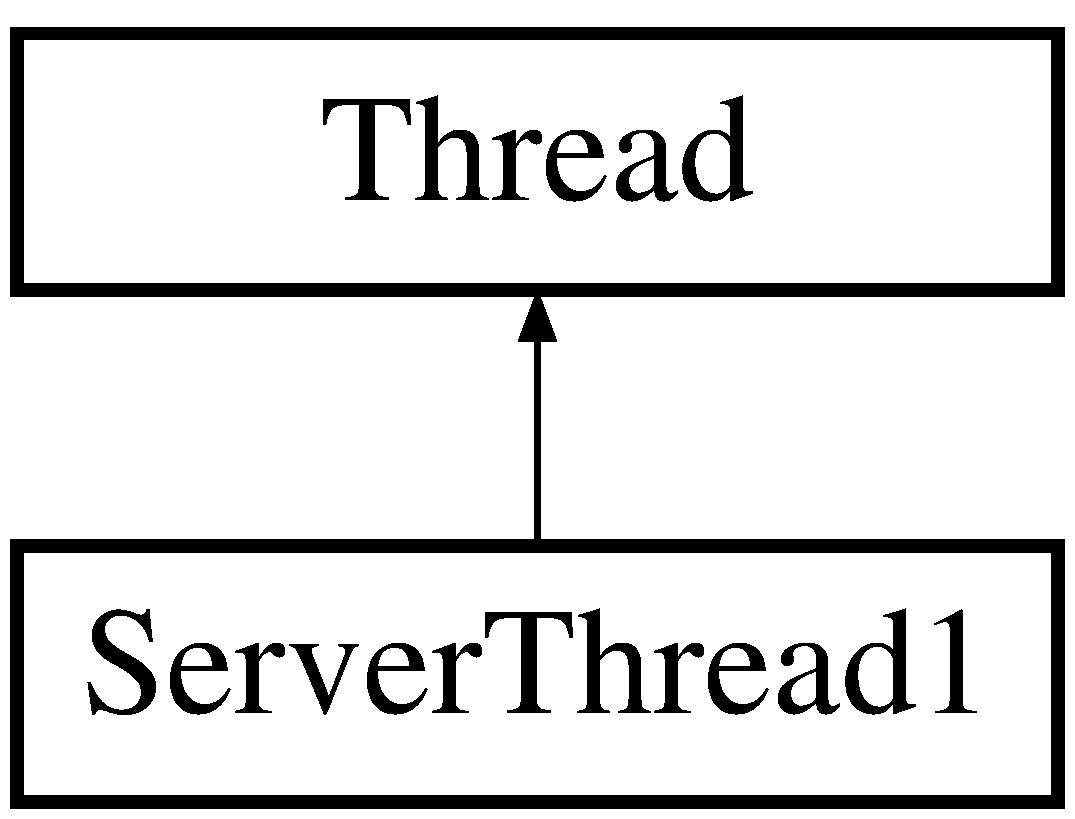
\includegraphics[height=2.000000cm]{class_server_thread1}
\end{center}
\end{figure}
\subsection*{Public Member Functions}
\begin{DoxyCompactItemize}
\item 
{\bfseries Server\+Thread1} (String name)  throws I\+O\+Exception\hypertarget{class_server_thread1_ae29df115466a434608801b3c751def7d}{}\label{class_server_thread1_ae29df115466a434608801b3c751def7d}

\item 
void {\bfseries run} ()\hypertarget{class_server_thread1_ad91d48187f6e88a980d36b2182ec1c55}{}\label{class_server_thread1_ad91d48187f6e88a980d36b2182ec1c55}

\end{DoxyCompactItemize}
\subsection*{Static Public Member Functions}
\begin{DoxyCompactItemize}
\item 
static List$<$ Integer $>$ {\bfseries decode\+Byte\+Message} (byte\mbox{[}$\,$\mbox{]} b)\hypertarget{class_server_thread1_a81e7367f1e95b9e1ecdbbc8b5da526b7}{}\label{class_server_thread1_a81e7367f1e95b9e1ecdbbc8b5da526b7}

\end{DoxyCompactItemize}
\subsection*{Static Protected Attributes}
\begin{DoxyCompactItemize}
\item 
static Datagram\+Socket {\bfseries socket} = null\hypertarget{class_server_thread1_a99569f086bee535af8d46d6c6f4b46db}{}\label{class_server_thread1_a99569f086bee535af8d46d6c6f4b46db}

\end{DoxyCompactItemize}


\subsection{Detailed Description}
\hyperlink{class_server_thread1}{Server\+Thread1}. 

Runs on machine 2 and receives packets from \hyperlink{class_u_d_p_server_thread}{U\+D\+P\+Server\+Thread} running on machine 1. It then decodes these messages and stores them for the cursor thread to use. 

The documentation for this class was generated from the following file\+:\begin{DoxyCompactItemize}
\item 
Android\+Mouse/src/Server\+Thread1.\+java\end{DoxyCompactItemize}

\hypertarget{class_u_d_p_server}{}\section{U\+D\+P\+Server Class Reference}
\label{class_u_d_p_server}\index{U\+D\+P\+Server@{U\+D\+P\+Server}}


\hyperlink{class_u_d_p_server}{U\+D\+P\+Server} class.  


\subsection*{Static Public Member Functions}
\begin{DoxyCompactItemize}
\item 
static void {\bfseries main} (String\mbox{[}$\,$\mbox{]} args)  throws I\+O\+Exception\hypertarget{class_u_d_p_server_a02e0cce3658b00026dc771ea5ef2c345}{}\label{class_u_d_p_server_a02e0cce3658b00026dc771ea5ef2c345}

\end{DoxyCompactItemize}
\subsection*{Static Public Attributes}
\begin{DoxyCompactItemize}
\item 
static boolean {\bfseries running}\hypertarget{class_u_d_p_server_a4ea441d611623c0c772dd672f2dbdee8}{}\label{class_u_d_p_server_a4ea441d611623c0c772dd672f2dbdee8}

\item 
static int {\bfseries x\+Degrees}\hypertarget{class_u_d_p_server_a688dd8ca331852530eb2512ce84fa97c}{}\label{class_u_d_p_server_a688dd8ca331852530eb2512ce84fa97c}

\item 
static int {\bfseries y\+Degrees}\hypertarget{class_u_d_p_server_a79f1b6e14ce248b34f241fde2908a17c}{}\label{class_u_d_p_server_a79f1b6e14ce248b34f241fde2908a17c}

\item 
static boolean {\bfseries message\+Received} = false\hypertarget{class_u_d_p_server_aec0aecab61ce5f57b5642cc5fa2cc52c}{}\label{class_u_d_p_server_aec0aecab61ce5f57b5642cc5fa2cc52c}

\item 
static boolean {\bfseries flag} = true\hypertarget{class_u_d_p_server_a35aa40c2624191ef9f0e00d8500c3f3a}{}\label{class_u_d_p_server_a35aa40c2624191ef9f0e00d8500c3f3a}

\item 
static String {\bfseries secondary\+IP}\hypertarget{class_u_d_p_server_adac7169a538dfe95223b9db39dacdaf5}{}\label{class_u_d_p_server_adac7169a538dfe95223b9db39dacdaf5}

\item 
static int {\bfseries user\+Count}\hypertarget{class_u_d_p_server_aa5e77770fdd1b55bb63f3252d4881170}{}\label{class_u_d_p_server_aa5e77770fdd1b55bb63f3252d4881170}

\end{DoxyCompactItemize}


\subsection{Detailed Description}
\hyperlink{class_u_d_p_server}{U\+D\+P\+Server} class. 

Main class, gets user inputs to determine machine number and secondary server IP if necessary, then starts the correct \hyperlink{class_u_d_p_server}{U\+D\+P\+Server} thread as well as the cursor thread. It then waits for a user input and then terminates. 

The documentation for this class was generated from the following file\+:\begin{DoxyCompactItemize}
\item 
Android\+Mouse/src/U\+D\+P\+Server.\+java\end{DoxyCompactItemize}

\hypertarget{class_u_d_p_server_thread}{}\section{U\+D\+P\+Server\+Thread Class Reference}
\label{class_u_d_p_server_thread}\index{U\+D\+P\+Server\+Thread@{U\+D\+P\+Server\+Thread}}


U\+P\+Server\+Thread class.  


Inheritance diagram for U\+D\+P\+Server\+Thread\+:\begin{figure}[H]
\begin{center}
\leavevmode
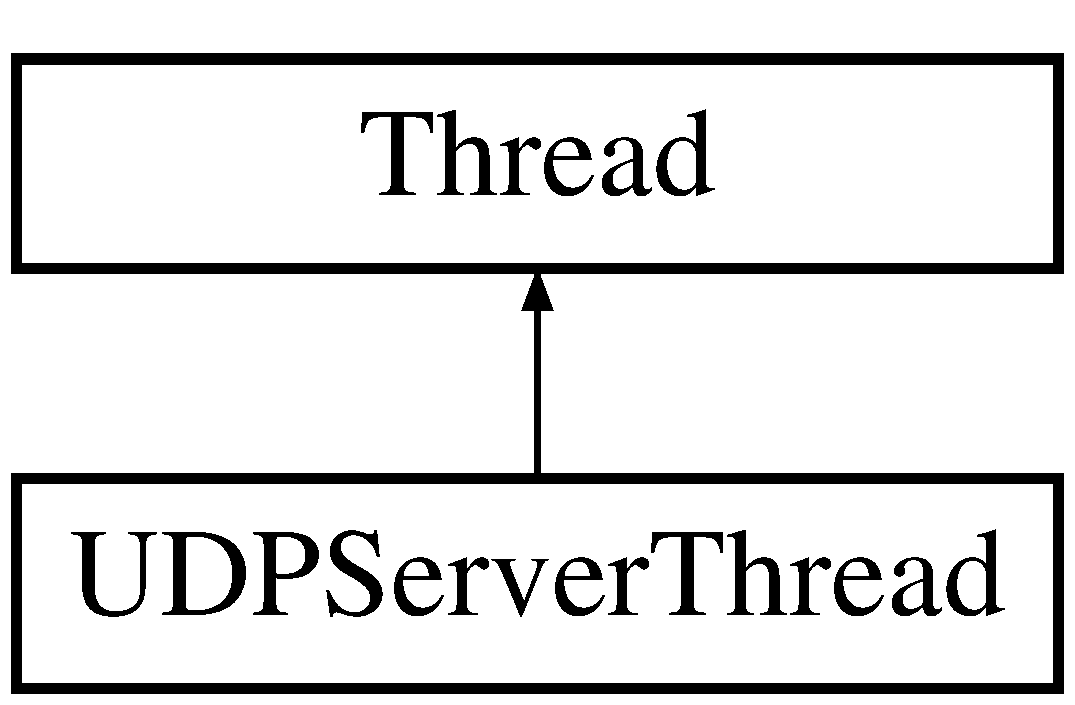
\includegraphics[height=2.000000cm]{class_u_d_p_server_thread}
\end{center}
\end{figure}
\subsection*{Public Member Functions}
\begin{DoxyCompactItemize}
\item 
{\bfseries U\+D\+P\+Server\+Thread} (String name)  throws I\+O\+Exception\hypertarget{class_u_d_p_server_thread_a1ec2d026557fc3be980f97de1564ae0a}{}\label{class_u_d_p_server_thread_a1ec2d026557fc3be980f97de1564ae0a}

\item 
void {\bfseries run} ()\hypertarget{class_u_d_p_server_thread_a6745593688fac3eb6098232d78f4cd01}{}\label{class_u_d_p_server_thread_a6745593688fac3eb6098232d78f4cd01}

\end{DoxyCompactItemize}
\subsection*{Static Public Member Functions}
\begin{DoxyCompactItemize}
\item 
static List$<$ Integer $>$ \hyperlink{class_u_d_p_server_thread_af5c340f848a87a00e26aa3099a815265}{decode\+Byte\+Message} (byte\mbox{[}$\,$\mbox{]} b)
\begin{DoxyCompactList}\small\item\em decode\+Byte\+Message. \end{DoxyCompactList}\end{DoxyCompactItemize}
\subsection*{Static Protected Attributes}
\begin{DoxyCompactItemize}
\item 
static Datagram\+Socket {\bfseries socket1} = null\hypertarget{class_u_d_p_server_thread_a77619fbca35791a3a9640e4c1996a1aa}{}\label{class_u_d_p_server_thread_a77619fbca35791a3a9640e4c1996a1aa}

\item 
static Datagram\+Socket {\bfseries socket2} = null\hypertarget{class_u_d_p_server_thread_aae235972e90c4e6b27801ad577526cae}{}\label{class_u_d_p_server_thread_aae235972e90c4e6b27801ad577526cae}

\end{DoxyCompactItemize}


\subsection{Detailed Description}
U\+P\+Server\+Thread class. 

This class opens sockets and receives packets from Android devices. The IP address of the packet is checked. If it is a new IP, a new user object is created, assigned a team, and added to the users list. If the user is assigned to the other team, the data packet will be sent to the secondary server. Otherwise, the packet is decoded and the data is used to move the mouse cursor. 

\subsection{Member Function Documentation}
\index{U\+D\+P\+Server\+Thread@{U\+D\+P\+Server\+Thread}!decode\+Byte\+Message@{decode\+Byte\+Message}}
\index{decode\+Byte\+Message@{decode\+Byte\+Message}!U\+D\+P\+Server\+Thread@{U\+D\+P\+Server\+Thread}}
\subsubsection[{\texorpdfstring{decode\+Byte\+Message(byte[] b)}{decodeByteMessage(byte[] b)}}]{\setlength{\rightskip}{0pt plus 5cm}static List$<$Integer$>$ U\+D\+P\+Server\+Thread.\+decode\+Byte\+Message (
\begin{DoxyParamCaption}
\item[{byte\mbox{[}$\,$\mbox{]}}]{b}
\end{DoxyParamCaption}
)\hspace{0.3cm}{\ttfamily [static]}}\hypertarget{class_u_d_p_server_thread_af5c340f848a87a00e26aa3099a815265}{}\label{class_u_d_p_server_thread_af5c340f848a87a00e26aa3099a815265}


decode\+Byte\+Message. 

Takes a byte message and returns a list of two integer values (pitch and roll) 

The documentation for this class was generated from the following file\+:\begin{DoxyCompactItemize}
\item 
Android\+Mouse/src/U\+D\+P\+Server\+Thread.\+java\end{DoxyCompactItemize}

\hypertarget{class_users}{}\section{Users Class Reference}
\label{class_users}\index{Users@{Users}}


\hyperlink{class_users}{Users} class.  


\subsection*{Public Member Functions}
\begin{DoxyCompactItemize}
\item 
{\bfseries Users} (String ip, int team)\hypertarget{class_users_a5da8355fe6af294477914f55271a1fb5}{}\label{class_users_a5da8355fe6af294477914f55271a1fb5}

\end{DoxyCompactItemize}
\subsection*{Public Attributes}
\begin{DoxyCompactItemize}
\item 
String {\bfseries ip}\hypertarget{class_users_a451f187d7cf746ea23161eebba077408}{}\label{class_users_a451f187d7cf746ea23161eebba077408}

\item 
int {\bfseries team}\hypertarget{class_users_ae8934893539c13c7eee3a7e8385a5f55}{}\label{class_users_ae8934893539c13c7eee3a7e8385a5f55}

\end{DoxyCompactItemize}


\subsection{Detailed Description}
\hyperlink{class_users}{Users} class. 

Used to keep track of IP and team number of individual users. 

The documentation for this class was generated from the following file\+:\begin{DoxyCompactItemize}
\item 
Android\+Mouse/src/Users.\+java\end{DoxyCompactItemize}

%--- End generated contents ---

% Index
\backmatter
\newpage
\phantomsection
\clearemptydoublepage
\addcontentsline{toc}{chapter}{Index}
\printindex

\end{document}
